\documentclass[border=12pt]{standalone}
\usepackage[T1]{fontenc}
\usepackage{helvet}
\renewcommand{\familydefault}{\sfdefault}
\usepackage{amsmath}
\usepackage{tikz}
\usetikzlibrary{positioning,arrows.meta,calc,fit,backgrounds,shapes.geometric,shapes.misc}

% palette
\definecolor{spinefill}{RGB}{232,234,238}
\definecolor{spinedraw}{RGB}{110,118,130}
\definecolor{liverfill}{RGB}{246,247,249}
\definecolor{liverdraw}{RGB}{168,175,184}
\definecolor{teald}{RGB}{13,110,122}
\definecolor{tealfill}{RGB}{223,239,240}
\definecolor{amber}{RGB}{193,118,18}
\definecolor{amberfill}{RGB}{250,240,222}
\definecolor{inkc}{RGB}{33,38,46}
\definecolor{salmon}{RGB}{193,110,95}
\definecolor{salmonfill}{RGB}{244,225,220}

% badges
\newcommand{\bnew}{\colorbox{teald}{\textcolor{white}{\scriptsize\bfseries NEW}}\hspace{2pt}}
\newcommand{\bchg}{\colorbox{amber}{\textcolor{white}{\scriptsize\bfseries CHANGED}}\hspace{2pt}}

\begin{document}
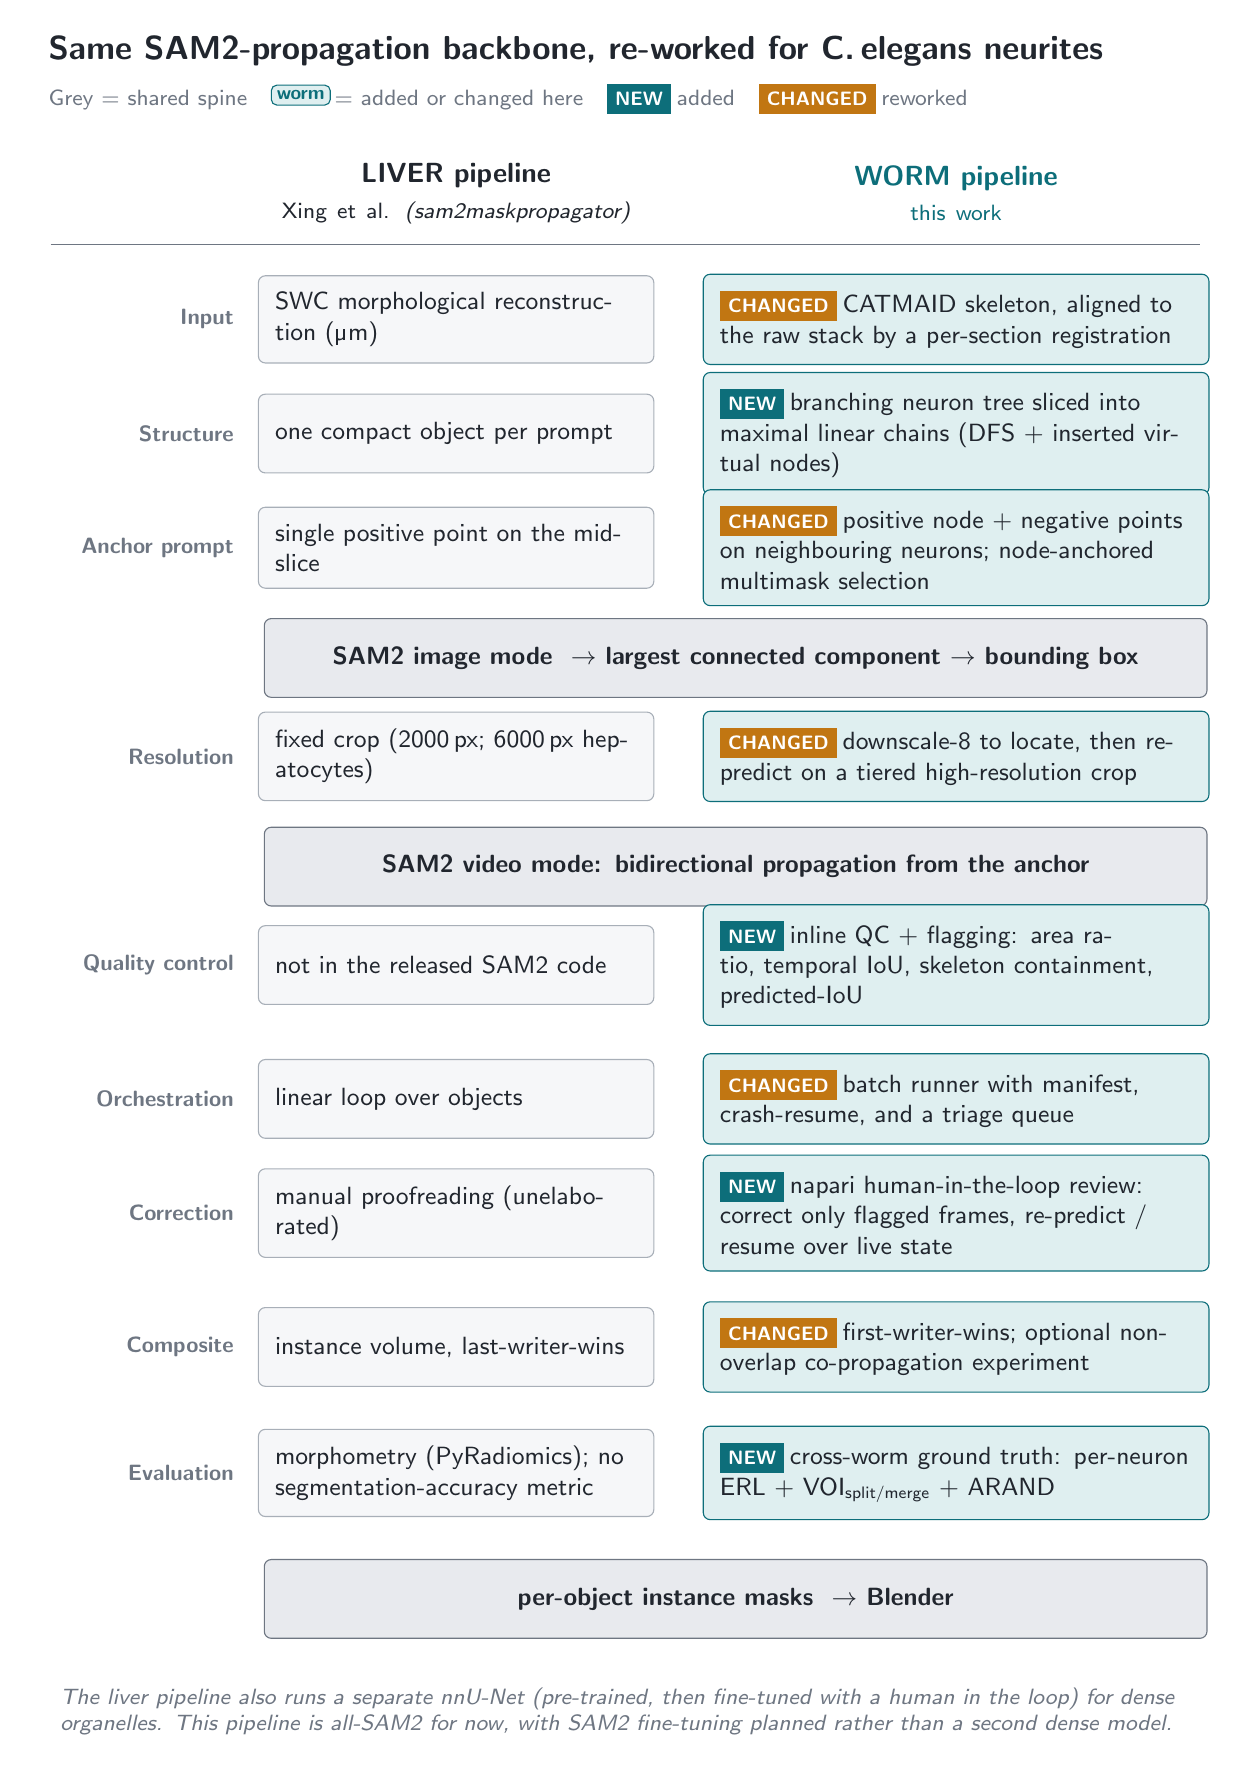
\begin{tikzpicture}[
  box/.style={rounded corners=2.5pt, draw, align=left, font=\small, inner sep=6pt, text=inkc, minimum height=1.0cm},
  liver/.style={box, fill=liverfill, draw=liverdraw, text width=4.6cm},
  worm/.style={box, fill=tealfill, draw=teald, text width=6.0cm},
  shared/.style={box, fill=spinefill, draw=spinedraw, text width=11.55cm, align=center, font=\small\bfseries},
  stage/.style={font=\footnotesize\bfseries, text=spinedraw, anchor=east, align=right, text width=2.5cm},
]
\def\lx{0}      % liver column centre
\def\wx{6.35}   % worm column centre
\def\sx{3.55}   % shared span centre
\def\stx{-2.7}  % stage label east edge

% ---- title ----
\node[align=left, font=\large\bfseries, text=inkc, anchor=west] at (-5.3,2.35)
  {Same SAM2-propagation backbone, re-worked for \emph{C.\,elegans} neurites};
\node[align=left, font=\footnotesize, text=spinedraw, anchor=west] at (-5.3,1.75)
  {Grey = shared spine \ \ \tikz\node[draw=teald,fill=tealfill,rounded corners=2pt,inner sep=2pt,font=\scriptsize\bfseries,text=teald]{worm};\,= added or changed here \ \ {\bnew}added \ \ {\bchg}reworked};

% ---- headers ----
\node[align=center, font=\bfseries, text=inkc, text width=4.6cm] (hL) at (\lx,0.55)
  {LIVER pipeline\\[1pt]\footnotesize\mdseries Xing et al. \textit{(sam2maskpropagator)}};
\node[align=center, font=\bfseries, text=teald, text width=6.0cm] (hW) at (\wx,0.55)
  {WORM pipeline\\[1pt]\footnotesize\mdseries this work};
\draw[spinedraw, line width=0.6pt] (-5.15,-0.1) -- (9.45,-0.1);

% helper rows
% row y positions
\foreach \i/\y in {1/-1.05,2/-2.5,3/-3.95,4/-5.4,5/-6.55,6/-8.0,7/-9.15,8/-10.85,9/-12.3,10/-14.15,11/-15.6,12/-17.35}{}

% 1 Input
\node[stage] at (\stx,-1.05) {Input};
\node[liver, anchor=center] at (\lx,-1.05) {SWC morphological reconstruction (\textmu m)};
\node[worm, anchor=center] at (\wx,-1.05) {\bchg CATMAID skeleton, aligned to the raw stack by a per-section registration};

% 2 Decompose
\node[stage] at (\stx,-2.5) {Structure};
\node[liver, anchor=center] at (\lx,-2.5) {one compact object per prompt};
\node[worm, anchor=center] at (\wx,-2.5) {\bnew branching neuron tree sliced into maximal linear chains (DFS $+$ inserted virtual nodes)};

% 3 Anchor prompt
\node[stage] at (\stx,-3.95) {Anchor prompt};
\node[liver, anchor=center] at (\lx,-3.95) {single positive point on the mid-slice};
\node[worm, anchor=center] at (\wx,-3.95) {\bchg positive node $+$ negative points on neighbouring neurons; node-anchored multimask selection};

% 4 shared
\node[shared, anchor=center] at (\sx,-5.35) {SAM2 image mode \ $\rightarrow$\ largest connected component\ $\rightarrow$\ bounding box};

% 5 Resolution
\node[stage] at (\stx,-6.6) {Resolution};
\node[liver, anchor=center] at (\lx,-6.6) {fixed crop (2000\,px; 6000\,px hepatocytes)};
\node[worm, anchor=center] at (\wx,-6.6) {\bchg downscale-8 to locate, then re-predict on a tiered high-resolution crop};

% 6 shared
\node[shared, anchor=center] at (\sx,-8.0) {SAM2 video mode: bidirectional propagation from the anchor};

% 7 QC
\node[stage] at (\stx,-9.25) {Quality control};
\node[liver, anchor=center] at (\lx,-9.25) {not in the released SAM2 code};
\node[worm, anchor=center] at (\wx,-9.25) {\bnew inline QC $+$ flagging: area ratio, temporal IoU, skeleton containment, predicted-IoU};

% 8 Orchestration
\node[stage] at (\stx,-10.95) {Orchestration};
\node[liver, anchor=center] at (\lx,-10.95) {linear loop over objects};
\node[worm, anchor=center] at (\wx,-10.95) {\bchg batch runner with manifest, crash-resume, and a triage queue};

% 9 Correction
\node[stage] at (\stx,-12.4) {Correction};
\node[liver, anchor=center] at (\lx,-12.4) {manual proofreading (unelaborated)};
\node[worm, anchor=center] at (\wx,-12.4) {\bnew napari human-in-the-loop review: correct only flagged frames, re-predict / resume over live state};

% 10 Composite
\node[stage] at (\stx,-14.1) {Composite};
\node[liver, anchor=center] at (\lx,-14.1) {instance volume, last-writer-wins};
\node[worm, anchor=center] at (\wx,-14.1) {\bchg first-writer-wins; optional non-overlap co-propagation experiment};

% 11 Evaluation
\node[stage] at (\stx,-15.7) {Evaluation};
\node[liver, anchor=center] at (\lx,-15.7) {morphometry (PyRadiomics); no segmentation-accuracy metric};
\node[worm, anchor=center] at (\wx,-15.7) {\bnew cross-worm ground truth: per-neuron ERL $+$ VOI$_{\text{split/merge}}$ $+$ ARAND};

% 12 shared
\node[shared, anchor=center] at (\sx,-17.3) {per-object instance masks \ $\rightarrow$\ Blender};

% ---- footnote ----
\node[align=left, font=\footnotesize\itshape, text=spinedraw, text width=14.3cm, anchor=north west] at (-5.15,-18.3)
  {The liver pipeline also runs a separate nnU-Net (pre-trained, then fine-tuned with a human in the loop) for dense organelles. This pipeline is all-SAM2 for now, with SAM2 fine-tuning planned rather than a second dense model.};

\end{tikzpicture}
\end{document}
